\section{Background and Related Work}
\label{sec:back}

\label{sec:back-discrimination}
\noindent 
Discrimination, defined as adverse behaviors, negative judgment, or unfair treatment towards a person, can be an uncontrollable and unpredictable stressor, and as such can severely influence health and well-being \citep{Williams:2009}. However, risk factors and protective factors often explain why similar experiences impact people differently \citep{SeridoAlmeidaWethington:2004}.  Stress is not evenly distributed. People with less privileged statuses have  greater exposure to stressors such as discrimination; further, stress proliferation increases their risk of subsequent cascades of stress exposure and  lessens protective resources, deepening negative impact and outcome disparities (Pearlin et al., 2005).

In terms of the responses it elicits and  health and functioning outcomes, the effect of discrimination can be studied within a stress and coping framework \citep{Pearlin:1999}. Ong \etal (\citeyear{Ong:2009}) apply this framework to  study  response to incidents of discrimination, using it to account for stress response variability based on the previous and current contexts of their lives. They discuss mechanisms through which chronic discrimination is linked to both daily discrimination as well as other negative events, which cumulatively lead to outcomes such as psychological distress. In a  study of  174 African American doctoral students, they demonstrated the relationship between both chronic and daily discrimination to distress; they showed that chronic exposure to discrimination exacerbates reactions to daily discrimination incidents, and that chronic and daily discrimination as well as other negative events each contribute to distress. Since then, other works have demonstrated a clear relationship between discrimination and stress (\eg \cite{Pieterse:2007}).  \paula{check my editing above; my effort here is to lay out some additional concepts that we will later use. Note I added a cite}
Because of discrimination's links to stress, it is not surprising that it can affect both physical and psychological well-being, as we now discuss.

\paragraph{Physical Well-Being:}
\label{sec:back-discrimination-physical}
When discrimination triggers a stress response, it can cause physiological changes such as heightened blood pressure, heart rate, and cortisol secretions \citep{Brondolo:2008, Steffen:2003, Smart:2010}; these can lead to serious conditions such as heart disease (\eg \cite{Marshall:1997, Cohen:1994}). Should it happen repeatedly, discrimination increases reactivity to stressful situations \citep{GuyllMatthewsBrom-berger:2001} and weakens the body's protective resources, thus increasing the risk of illness similar to other forms of cumulative stress \citep{GeeSpencerChenTakeuchi:2007}. Additionally, discrimination is directly correlated with more unhealthy behavior (\eg smoking, drinking, substance use \citep{LandrineKlonoff:1996, MartinTuchRoman:2003}). 

\paragraph{Psychological Well-Being:}
\label{sec:back-discrimination-mental}
The association between exposure to discrimination and mental health is well supported by empirical evidence \citep{Pascoe:2009} as well as large-scale population studies \citep{Kessler:1999}. Not only is discrimination directly associated with higher levels of depression, anxiety, and psychological distress in general, it is negatively correlated with identifiers of healthy psyche, such as positive affect \citep{Schmitt:2014}. The magnitude of the associations is larger for negative health outcomes (\eg depression \citep{Schmitt:2014}) and is comparable to major stressors such as sexual assault or combat experience \citep{Kessler:1999}. 
Consistent with Ong, \etal's (\citeyear{Ong:2009}) application of the stress and coping framework to discrimination, responses differ depending on factors like prior exposure  \citep{Kessler:1999}. 

\subsection{Open Questions}
\noindent The relationships documented in the literature are summarized in Figure~\ref{fig:model}.  A great deal of evidence shows that both daily and cumulative discrimination are linked to stress and thus impact physical and psychological well-being.  However, a unified model that relates short-term behavior to long-term outcomes still does not exist. Although \citet{Ong:2009} propose multiple models, their work focuses only on self-reported measures. In addition, it is not yet clear how discrimination relates specifically to academic outcomes such as grades and retention. Finally, no prior work has quantified the impact of risk factors and protective factors on these relationships. A better understanding of the relationship between short-term changes and long-term outcomes can help us to design more effective interventions and improve our ability to model the overall effects of discrimination.


\begin{figure}
    \centering
    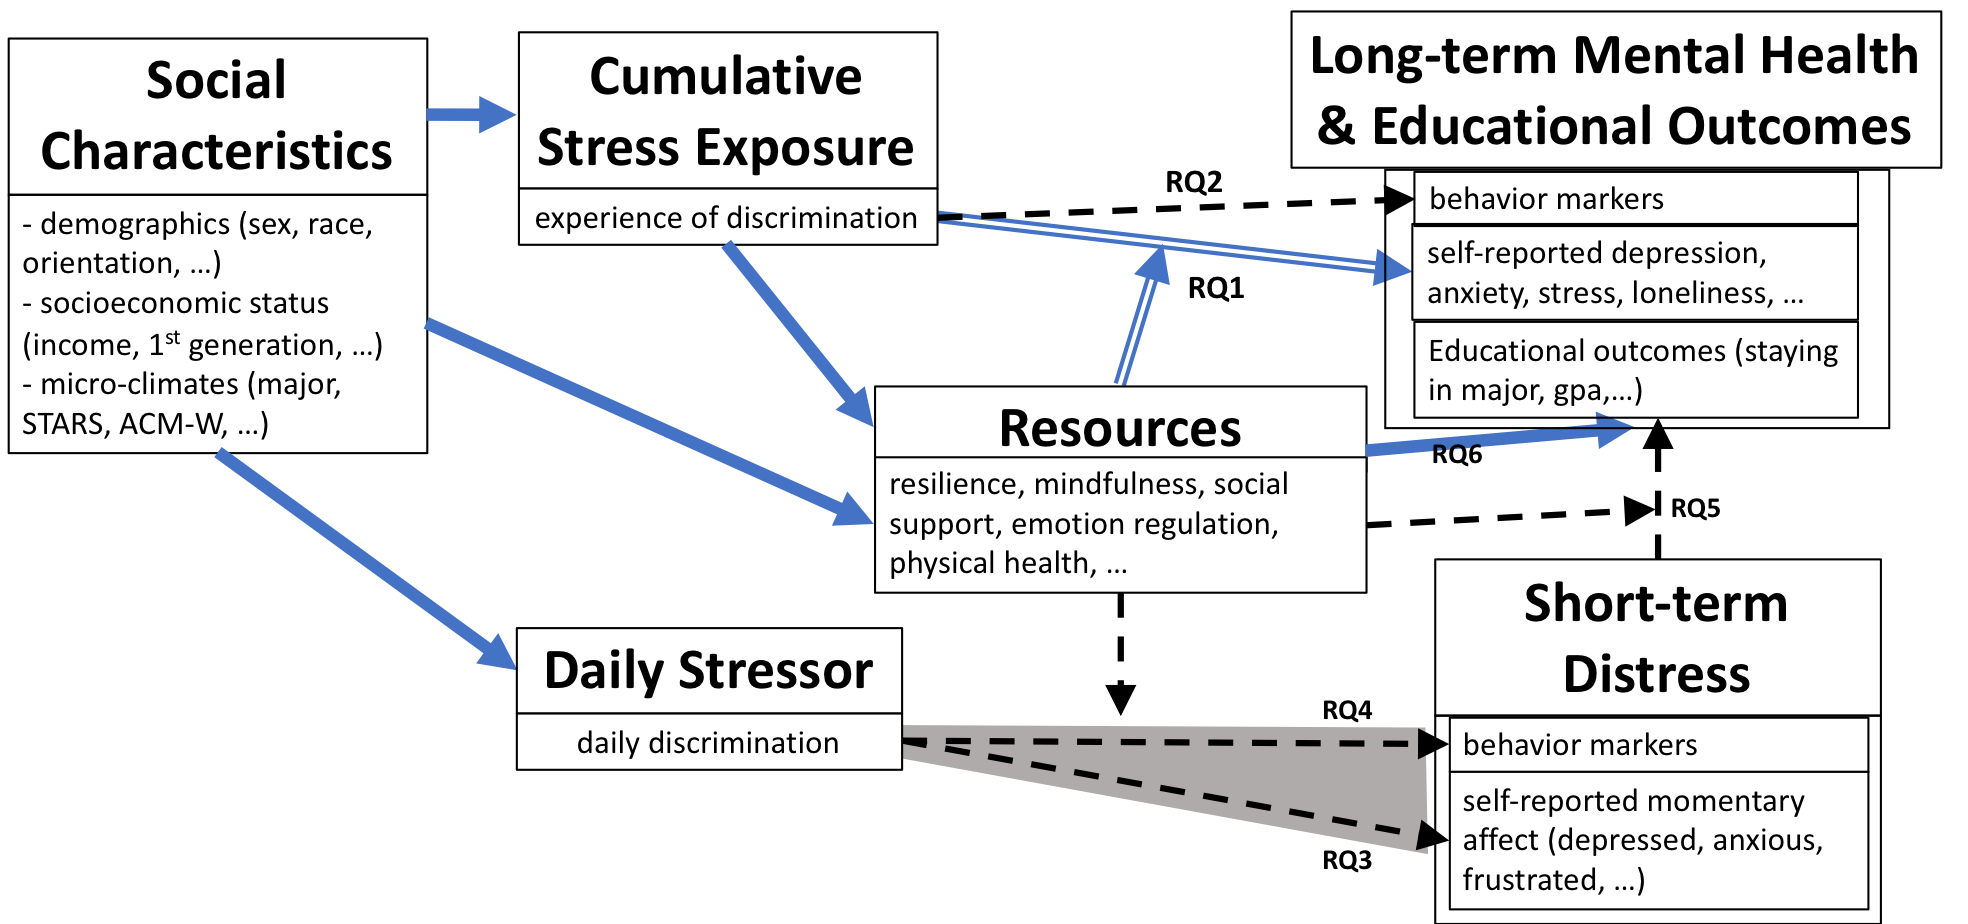
\includegraphics[width=5.2in]{img/stress-process-model.png}
    \caption[Stress process model of discrimination]{Stress process model of short- and long-term impact of discrimination. \jen{add rqs; remove highlights: The highlighted links are specifically examined in the present work.} Thick blue arrows have been studied in the past. We are reproducing the ones with double lines. Dashed arrows have not been fully examined to the best of our knowledge, particularly in relation to behavior markers. When a moderating impact is applicable to multiple arrows, we have enclosed the arrows in a gray box to minimize clutter.
    }
    \label{fig:model}
\end{figure}

Thus, we have the following research questions. In terms of long-term differences we specifically ask: %\yasaman{Analysis of the global behavior patterns and discrimination is similar to the analysis in paper tracking depression dynamics by Campbell’s group in UbiComp’18 that looked at PHQ8 and behavior patterns.}

\begin{enumerate}[start=1,label={\bfseries RQ\arabic*}, leftmargin=1.5cm]
    \item \label{itm:rq-long-outcome} What are the differences in mental health (\eg anxiety, depression, or loneliness) between people who experience discrimination and people who do not, accounting for contributions of cumulative discrimination and resources.
    \item \label{itm:rq-long-behavior} Do these differences also exist at the level of global behavior patterns (\ie behaviors aggregated for the duration of the study) as captured by phone and  wearable devices?
\end{enumerate}

Answers to these questions would allow us to establish differences in mental health based on cumulative discriminatory experiences. 

Turning to short-term impact, our questions are below. Should there be any changes we will specifically explore their strength and duration.

\begin{enumerate}[start=3,label={\bfseries RQ\arabic*}, leftmargin=1.5cm]
    \item \label{itm:rq-short-outcome} What are the differences in self-reported daily affect in the presence and absence of reports of discrimination? %\yasaman{to be later considered: differences in daily stress health behavior}
    \item \label{itm:rq-short-behavior} Are there differences at the level of behavior patterns captured by phone and  wearable devices as a function of discrimination exposure?
\end{enumerate}

Responses to \ref{itm:rq-short-outcome} and \ref{itm:rq-short-behavior} would provide much needed insights into psychological and behavioral changes that follow unfair treatment, which would justify the need for the future study of the mediating impact of short-term distress on deteriorated mental health in the long-term.

\begin{enumerate}[start=5,label={\bfseries RQ\arabic*}, leftmargin=1.5cm]
\item \label{itm:rq-short-long} We also wish to understand the relationship between short term and long term changes. Thus we will study the relationship between short term behavior change and long term change over the course of the four years of the study, such as GPA and staying in major. 
\item \label{itm:rq-short-long-mediation} Finally, we will study the impact of mediating factors that cumulative stress and micro-climates can influence such as resilience and social support on these long-term outcomes. 

\end{enumerate}


For each observed relationship, we consider several important aspects. First, it is important to know whether we have \textit{confidence} in the observations. This can be expressed in terms of \textit{p}-values while accounting for multiple comparisons. 
Second, it is important to quantify the \textit{magnitude} of the relationship. This can be expressed in terms of effect sizes or model parameters (\eg regression coefficients).
Finally, it is important to quantify the \textit{length of time} over which the impact is visible (short-term analysis only). This can be captured by looking at the decay in confidence over time.

%Examining both long-term and short-term measures we ask: how do risk / protective factors moderate the relationship? \yasaman{we ended up not looking at risk and protective factors for short-term analysis} % Additionally, we consider correlations between subjective self-reports and objective metrics obtained from phone / wearable data. \yasaman{this is basically done during behavior metric selection.}

